\chapter[Ferramentas utilizadas]{Ferramentas utilizadas}
\addcontentsline{toc}{chapter}{Ferramentas utilizadas}
\markboth{Ferramentas utilizadas}{Ferramentas utilizadas}

O desenvolvimento do jogo contou com o apoio de ferramentas específicas, selecionadas pela sua capacidade de atender às demandas do projeto. As principais ferramentas utilizadas foram:

\section{Aseprite}

O Aseprite foi utilizado para criar os elementos gráficos do jogo, como sprites de personagens, veículos e efeitos visuais. Essa ferramenta é amplamente reconhecida no desenvolvimento de jogos 2D devido à sua interface intuitiva e recursos especializados em \textit{pixel art} \cite{aseprite}.

\begin{figure}[htbp]
    \centering
    \caption{sofware aseprite}
    \label{fig:asesprite}
    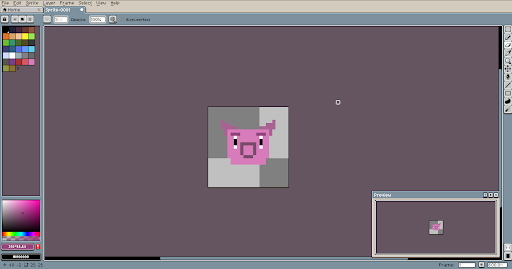
\includegraphics[width=0.7\textwidth]{figuras/asesprite.png}
    \legend{Fonte: Elaboração própria.}
\end{figure}

\section{Godot e GDScript}

A engine Godot foi escolhida como plataforma principal para o desenvolvimento do jogo, devido à sua versatilidade e comunidade ativa. O uso do GDScript, uma linguagem integrada à engine, permitiu a implementação de mecânicas e sistemas com agilidade. A Godot oferece recursos nativos para jogos 2D, como sistemas de colisão e animações, que foram essenciais para o projeto \cite{godot}.

Além disso, a Godot fornece suporte para múltiplas plataformas, abrangendo os principais sistemas operacionais e navegadores web.

\begin{figure}[htbp]
    \centering
    \caption{software Godot}
    \label{fig:godot}
    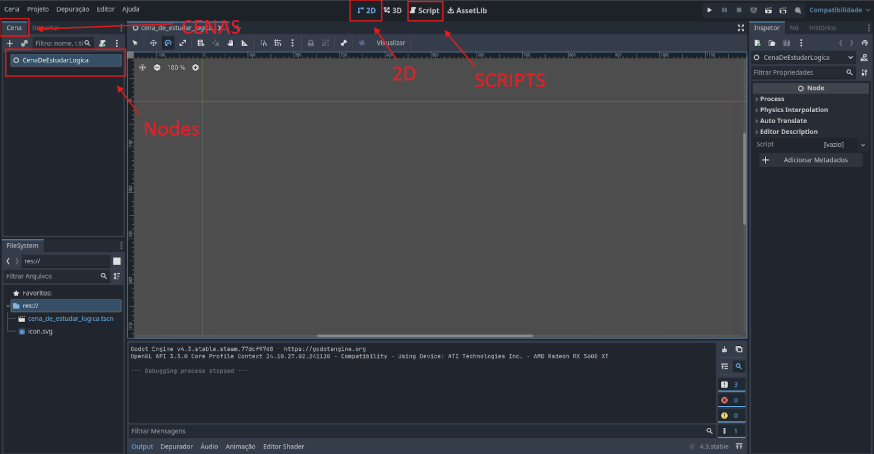
\includegraphics[width=0.7\textwidth]{figuras/godot-use.png}
    \legend{Fonte: Elaboração própria.}
\end{figure}

\section{Trello}

O Trello foi utilizado para gerenciar as tarefas do projeto, permitindo organização visual e controle do progresso em cada sprint. Essa ferramenta ajudou a manter o fluxo de trabalho alinhado com os princípios do Scrum.

Ao utilizar essas ferramentas em conjunto, foi possível criar um ambiente de desenvolvimento eficiente, onde cada etapa do processo contribuiu para o alcance dos objetivos do projeto.

\section{GitHub}

O GitHub foi utilizado para gerenciar as versões do projeto e fazer backups na nuvem. Ele permitiu acompanhar o progresso do trabalho, facilitando o controle das mudanças feitas no código e garantindo que o projeto estivesse sempre seguro e acessível. O repositório com o código-fonte está disponível no \textit{Anexo A}.

